% case-studies.tex
% Section 5: Pedagogical Case Studies

%%%%%%%%%%%%%%%%%%%%
\section{Pedagogical Case Studies}
%%%%%%%%%%%%%%%%%%%%

%%%%%%%%%%%%%%%%%%%%
\begin{frame}{Case Study Overview}
  \begin{center}
    \textbf{Deep-Dive Examples for Teaching Conceptual Understanding}
  \end{center}
  
  \vspace{0.5cm}
  
  \begin{enumerate}
    \item \textbf{Why C Has Undefined Behavior} --- History + Optimization Rationale
    \item \textbf{How \texttt{malloc}/\texttt{free} Work} --- Fragmentation vs. Speed
    \item \textbf{Java Lambda Desugaring} --- \texttt{invokedynamic} Mechanism
    \item \textbf{C Standard Library Design} --- 1970s Constraints
    \item \textbf{VLA Deprecation \& Large Projects} --- Security + Organization
  \end{enumerate}
  
  \vspace{0.3cm}
  
  \begin{block}{Pedagogical Goal}
    Each case study connects \textit{history} $\rightarrow$ \textit{rationale} $\rightarrow$ \textit{modern practice}.
  \end{block}
  
  % Speaker note: These case studies form the core of deep understanding
\end{frame}
%%%%%%%%%%%%%%%%%%%%

%%%%%%%%%%%%%%%%%%%%
\begin{frame}[fragile]{Case Study 1: Why C Has Undefined Behavior}
  \textbf{Historical Context (Dennis Ritchie, 1993)}
  
  \begin{quote}
    ``C is quirky, flawed, and an enormous success.''
  \end{quote}
  
  \begin{columns}[T]
    \begin{column}{0.48\textwidth}
      \textbf{Origins of UB:}
      \begin{itemize}
        \item \textbf{Portability} --- Ran on diverse hardware
        \item \textbf{Performance} --- No mandatory checks
        \item \textbf{Freedom} --- Compiler knows best
      \end{itemize}
    \end{column}
    \begin{column}{0.48\textwidth}
      \textbf{C99 Rationale Categories:}
      \begin{itemize}
        \item \textbf{Undefined} --- Anything can happen
        \item \textbf{Unspecified} --- Choice not documented
        \item \textbf{Implementation-defined} --- Documented choice
      \end{itemize}
    \end{column}
  \end{columns}
  
  \vspace{0.2cm}
  
  \begin{block}{Compiler Optimization via UB}
\begin{verbatim}
int x = *p;
if (p == NULL) { ... }  // Compiler removes this!
\end{verbatim}
    \textit{After dereferencing, p cannot be NULL (or UB already occurred).}
  \end{block}
  
  % Speaker note: Reference C99 Rationale document Section 4
\end{frame}
%%%%%%%%%%%%%%%%%%%%

%%%%%%%%%%%%%%%%%%%%
\begin{frame}[fragile]{Case Study 2: How \texttt{malloc}/\texttt{free} Work}
  \textbf{Memory Allocator Design Trade-offs}
  
  \begin{columns}[T]
    \begin{column}{0.48\textwidth}
      \begin{center}
        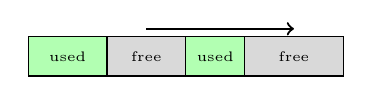
\begin{tikzpicture}[scale=0.5]
          \draw[fill=green!30] (0,0) rectangle (2,1);
          \node at (1,0.5) {\tiny used};
          \draw[fill=gray!30] (2,0) rectangle (4,1);
          \node at (3,0.5) {\tiny free};
          \draw[fill=green!30] (4,0) rectangle (5.5,1);
          \node at (4.75,0.5) {\tiny used};
          \draw[fill=gray!30] (5.5,0) rectangle (8,1);
          \node at (6.75,0.5) {\tiny free};
          \draw[->, thick] (3, 1.2) -- (6.75, 1.2);
        \end{tikzpicture}
      \end{center}
      
      \textbf{Strategies:} First-fit, Best-fit, Buddy system, Slab allocator
    \end{column}
    \begin{column}{0.48\textwidth}
      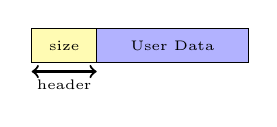
\begin{tikzpicture}[scale=0.55]
        \draw[fill=yellow!30] (0,0) rectangle (1.5,0.8);
        \node at (0.75,0.4) {\tiny size};
        \draw[fill=blue!30] (1.5,0) rectangle (5,0.8);
        \node at (3.25,0.4) {\tiny User Data};
        \draw[<->, thick] (0, -0.2) -- (1.5, -0.2);
        \node at (0.75, -0.5) {\tiny header};
      \end{tikzpicture}
      
      \textbf{Security:} Corrupting metadata enables exploits!
    \end{column}
  \end{columns}
  
  \vspace{0.3cm}
  
  \begin{block}{glibc Implementation}
    Uses bins for different sizes, thread-local caches, and \texttt{mmap} for large allocations. Understanding internals explains buffer overflow vulnerabilities.
  \end{block}
  
  % Speaker note: Reference glibc manual; connect to Java GC trade-offs
\end{frame}
%%%%%%%%%%%%%%%%%%%%

%%%%%%%%%%%%%%%%%%%%
\begin{frame}[fragile]{Case Study 3: Java Lambda Desugaring}
  \textbf{From Source to Bytecode}
  
  \begin{columns}[T]
    \begin{column}{0.48\textwidth}
      \begin{block}{Source Code}
\begin{verbatim}
int mult = 2;
IntUnaryOperator op =
    x -> x * mult;
\end{verbatim}
      \end{block}
      
      \textbf{What JVM Does:}
      \begin{itemize}
        \item \texttt{invokedynamic} instruction
        \item \texttt{LambdaMetafactory} creates class
        \item Captured vars become fields
      \end{itemize}
    \end{column}
    \begin{column}{0.48\textwidth}
      \begin{block}{Equivalent Class}
\begin{verbatim}
class Lambda$$1 {
  final int mult;
  int apply(int x) {
    return x * mult;
  }
}
\end{verbatim}
      \end{block}
      
      \textbf{Benefits:} No class file overhead, JVM can inline, explains ``effectively final'' requirement.
    \end{column}
  \end{columns}
  
  % Speaker note: Explains why captured variables must be effectively final
\end{frame}
%%%%%%%%%%%%%%%%%%%%

%%%%%%%%%%%%%%%%%%%%
\begin{frame}{Case Study 4: C Standard Library Design}
  \textbf{1970s Constraints That Shaped the Library}
  
  \begin{columns}[T]
    \begin{column}{0.48\textwidth}
      \textbf{Hardware Constraints:}
      \begin{itemize}
        \item Limited memory (64KB typical)
        \item Slow I/O devices
        \item No memory protection
        \item Diverse architectures
      \end{itemize}
    \end{column}
    \begin{column}{0.48\textwidth}
      \textbf{Design Decisions:}
      \begin{itemize}
        \item Buffered I/O (\texttt{FILE *})
        \item No bounds checking
        \item Caller allocates buffers
        \item Error codes, not exceptions
      \end{itemize}
    \end{column}
  \end{columns}
  
  \vspace{0.3cm}
  
  \begin{block}{P.J. Plauger, ``The Standard C Library''}
    ``Each function aims to do one thing well, with minimal overhead.''
  \end{block}
  
  \textbf{Teaching Point:} Understanding constraints explains why \texttt{gets()} existed.
  
  % Speaker note: Reference Plauger's book for detailed design rationale
\end{frame}
%%%%%%%%%%%%%%%%%%%%

%%%%%%%%%%%%%%%%%%%%
\begin{frame}[fragile]{Case Study 5: VLA Deprecation \& Large Project Structure}
  \begin{columns}[T]
    \begin{column}{0.48\textwidth}
      \textbf{Why VLA Is Deprecated:}
      \begin{block}{VLA Example (C99)}
\begin{verbatim}
void process(int n) {
  int buffer[n]; // UB risk!
}
\end{verbatim}
      \end{block}
      
      \textbf{Problems:}
      \begin{itemize}
        \item Stack overflow (no bounds check)
        \item Security vulnerability
        \item C11 made optional
        \item CERT C forbids (ARR32-C)
      \end{itemize}
    \end{column}
    \begin{column}{0.48\textwidth}
      \textbf{Linux Kernel Style:}
\begin{verbatim}
- Tabs (8 spaces)
- 80 char lines
- No typedef for structs
- goto for cleanup
\end{verbatim}
      
      \textbf{Why?} Thousands of contributors need consistency, maintainability over cleverness.
    \end{column}
  \end{columns}
  
  \vspace{0.2cm}
  
  \textbf{Teaching Point:} Style guides exist for engineering reasons, not aesthetics.
  
  % Speaker note: Reference Google C++ Style Guide, Professional CMake
\end{frame}
%%%%%%%%%%%%%%%%%%%%
